% Created by tikzDevice version 0.12 on 2019-03-27 16:15:27
% !TEX encoding = UTF-8 Unicode
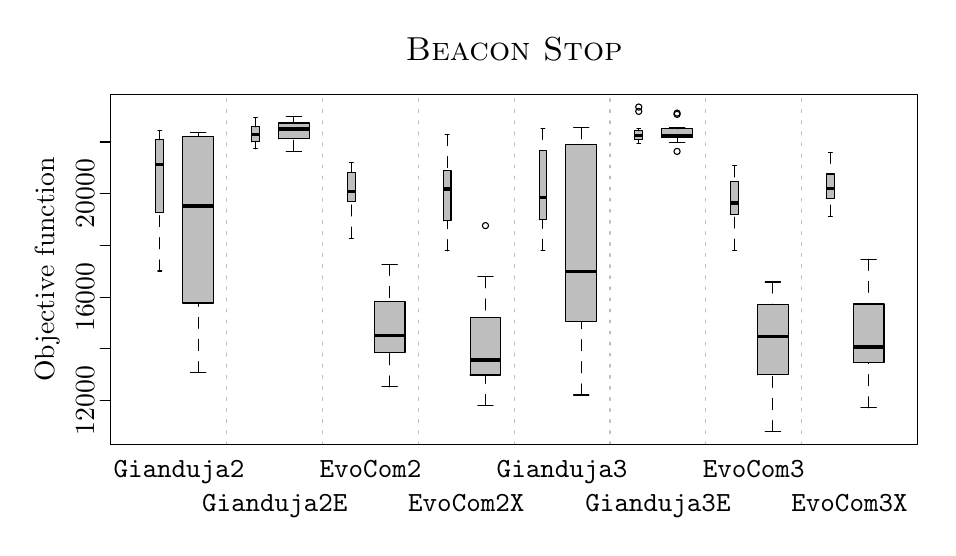
\begin{tikzpicture}[x=1pt,y=1pt]
\definecolor{fillColor}{RGB}{255,255,255}
\path[use as bounding box,fill=fillColor,fill opacity=0.00] (0,0) rectangle (325.21,180.67);
\begin{scope}
\path[clip] ( 30.00, 30.00) rectangle (321.61,156.67);
\definecolor{fillColor}{RGB}{190,190,190}

\path[fill=fillColor] ( 46.34,113.89) --
	( 49.11,113.89) --
	( 49.11,140.10) --
	( 46.34,140.10) --
	cycle;
\definecolor{drawColor}{RGB}{0,0,0}

\path[draw=drawColor,line width= 1.2pt,line join=round] ( 46.34,131.11) -- ( 49.11,131.11);

\path[draw=drawColor,line width= 0.4pt,dash pattern=on 4pt off 4pt ,line join=round,line cap=round] ( 47.72, 92.76) -- ( 47.72,113.89);

\path[draw=drawColor,line width= 0.4pt,dash pattern=on 4pt off 4pt ,line join=round,line cap=round] ( 47.72,143.56) -- ( 47.72,140.10);

\path[draw=drawColor,line width= 0.4pt,line join=round,line cap=round] ( 47.03, 92.76) -- ( 48.42, 92.76);

\path[draw=drawColor,line width= 0.4pt,line join=round,line cap=round] ( 47.03,143.56) -- ( 48.42,143.56);

\path[draw=drawColor,line width= 0.4pt,line join=round,line cap=round] ( 46.34,113.89) --
	( 49.11,113.89) --
	( 49.11,140.10) --
	( 46.34,140.10) --
	( 46.34,113.89);

\path[fill=fillColor] ( 56.03, 81.18) --
	( 67.11, 81.18) --
	( 67.11,141.32) --
	( 56.03,141.32) --
	cycle;

\path[draw=drawColor,line width= 1.2pt,line join=round] ( 56.03,116.18) -- ( 67.11,116.18);

\path[draw=drawColor,line width= 0.4pt,dash pattern=on 4pt off 4pt ,line join=round,line cap=round] ( 61.57, 56.01) -- ( 61.57, 81.18);

\path[draw=drawColor,line width= 0.4pt,dash pattern=on 4pt off 4pt ,line join=round,line cap=round] ( 61.57,142.66) -- ( 61.57,141.32);

\path[draw=drawColor,line width= 0.4pt,line join=round,line cap=round] ( 58.80, 56.01) -- ( 64.34, 56.01);

\path[draw=drawColor,line width= 0.4pt,line join=round,line cap=round] ( 58.80,142.66) -- ( 64.34,142.66);

\path[draw=drawColor,line width= 0.4pt,line join=round,line cap=round] ( 56.03, 81.18) --
	( 67.11, 81.18) --
	( 67.11,141.32) --
	( 56.03,141.32) --
	( 56.03, 81.18);

\path[fill=fillColor] ( 80.96,139.43) --
	( 83.73,139.43) --
	( 83.73,144.81) --
	( 80.96,144.81) --
	cycle;

\path[draw=drawColor,line width= 1.2pt,line join=round] ( 80.96,142.08) -- ( 83.73,142.08);

\path[draw=drawColor,line width= 0.4pt,dash pattern=on 4pt off 4pt ,line join=round,line cap=round] ( 82.34,136.89) -- ( 82.34,139.43);

\path[draw=drawColor,line width= 0.4pt,dash pattern=on 4pt off 4pt ,line join=round,line cap=round] ( 82.34,148.05) -- ( 82.34,144.81);

\path[draw=drawColor,line width= 0.4pt,line join=round,line cap=round] ( 81.65,136.89) -- ( 83.03,136.89);

\path[draw=drawColor,line width= 0.4pt,line join=round,line cap=round] ( 81.65,148.05) -- ( 83.03,148.05);

\path[draw=drawColor,line width= 0.4pt,line join=round,line cap=round] ( 80.96,139.43) --
	( 83.73,139.43) --
	( 83.73,144.81) --
	( 80.96,144.81) --
	( 80.96,139.43);

\path[fill=fillColor] ( 90.65,140.54) --
	(101.73,140.54) --
	(101.73,146.22) --
	( 90.65,146.22) --
	cycle;

\path[draw=drawColor,line width= 1.2pt,line join=round] ( 90.65,144.04) -- (101.73,144.04);

\path[draw=drawColor,line width= 0.4pt,dash pattern=on 4pt off 4pt ,line join=round,line cap=round] ( 96.19,136.00) -- ( 96.19,140.54);

\path[draw=drawColor,line width= 0.4pt,dash pattern=on 4pt off 4pt ,line join=round,line cap=round] ( 96.19,148.48) -- ( 96.19,146.22);

\path[draw=drawColor,line width= 0.4pt,line join=round,line cap=round] ( 93.42,136.00) -- ( 98.96,136.00);

\path[draw=drawColor,line width= 0.4pt,line join=round,line cap=round] ( 93.42,148.48) -- ( 98.96,148.48);

\path[draw=drawColor,line width= 0.4pt,line join=round,line cap=round] ( 90.65,140.54) --
	(101.73,140.54) --
	(101.73,146.22) --
	( 90.65,146.22) --
	( 90.65,140.54);

\path[fill=fillColor] (115.57,117.92) --
	(118.34,117.92) --
	(118.34,128.38) --
	(115.57,128.38) --
	cycle;

\path[draw=drawColor,line width= 1.2pt,line join=round] (115.57,121.53) -- (118.34,121.53);

\path[draw=drawColor,line width= 0.4pt,dash pattern=on 4pt off 4pt ,line join=round,line cap=round] (116.96,104.63) -- (116.96,117.92);

\path[draw=drawColor,line width= 0.4pt,dash pattern=on 4pt off 4pt ,line join=round,line cap=round] (116.96,131.81) -- (116.96,128.38);

\path[draw=drawColor,line width= 0.4pt,line join=round,line cap=round] (116.27,104.63) -- (117.65,104.63);

\path[draw=drawColor,line width= 0.4pt,line join=round,line cap=round] (116.27,131.81) -- (117.65,131.81);

\path[draw=drawColor,line width= 0.4pt,line join=round,line cap=round] (115.57,117.92) --
	(118.34,117.92) --
	(118.34,128.38) --
	(115.57,128.38) --
	(115.57,117.92);

\path[fill=fillColor] (125.27, 63.36) --
	(136.34, 63.36) --
	(136.34, 81.66) --
	(125.27, 81.66) --
	cycle;

\path[draw=drawColor,line width= 1.2pt,line join=round] (125.27, 69.37) -- (136.34, 69.37);

\path[draw=drawColor,line width= 0.4pt,dash pattern=on 4pt off 4pt ,line join=round,line cap=round] (130.81, 50.87) -- (130.81, 63.36);

\path[draw=drawColor,line width= 0.4pt,dash pattern=on 4pt off 4pt ,line join=round,line cap=round] (130.81, 95.14) -- (130.81, 81.66);

\path[draw=drawColor,line width= 0.4pt,line join=round,line cap=round] (128.04, 50.87) -- (133.57, 50.87);

\path[draw=drawColor,line width= 0.4pt,line join=round,line cap=round] (128.04, 95.14) -- (133.57, 95.14);

\path[draw=drawColor,line width= 0.4pt,line join=round,line cap=round] (125.27, 63.36) --
	(136.34, 63.36) --
	(136.34, 81.66) --
	(125.27, 81.66) --
	(125.27, 63.36);

\path[fill=fillColor] (150.19,110.86) --
	(152.96,110.86) --
	(152.96,129.07) --
	(150.19,129.07) --
	cycle;

\path[draw=drawColor,line width= 1.2pt,line join=round] (150.19,122.34) -- (152.96,122.34);

\path[draw=drawColor,line width= 0.4pt,dash pattern=on 4pt off 4pt ,line join=round,line cap=round] (151.58,100.05) -- (151.58,110.86);

\path[draw=drawColor,line width= 0.4pt,dash pattern=on 4pt off 4pt ,line join=round,line cap=round] (151.58,142.10) -- (151.58,129.07);

\path[draw=drawColor,line width= 0.4pt,line join=round,line cap=round] (150.88,100.05) -- (152.27,100.05);

\path[draw=drawColor,line width= 0.4pt,line join=round,line cap=round] (150.88,142.10) -- (152.27,142.10);

\path[draw=drawColor,line width= 0.4pt,line join=round,line cap=round] (150.19,110.86) --
	(152.96,110.86) --
	(152.96,129.07) --
	(150.19,129.07) --
	(150.19,110.86);

\path[fill=fillColor] (159.88, 55.15) --
	(170.96, 55.15) --
	(170.96, 76.07) --
	(159.88, 76.07) --
	cycle;

\path[draw=drawColor,line width= 1.2pt,line join=round] (159.88, 60.56) -- (170.96, 60.56);

\path[draw=drawColor,line width= 0.4pt,dash pattern=on 4pt off 4pt ,line join=round,line cap=round] (165.42, 44.13) -- (165.42, 55.15);

\path[draw=drawColor,line width= 0.4pt,dash pattern=on 4pt off 4pt ,line join=round,line cap=round] (165.42, 90.63) -- (165.42, 76.07);

\path[draw=drawColor,line width= 0.4pt,line join=round,line cap=round] (162.65, 44.13) -- (168.19, 44.13);

\path[draw=drawColor,line width= 0.4pt,line join=round,line cap=round] (162.65, 90.63) -- (168.19, 90.63);

\path[draw=drawColor,line width= 0.4pt,line join=round,line cap=round] (159.88, 55.15) --
	(170.96, 55.15) --
	(170.96, 76.07) --
	(159.88, 76.07) --
	(159.88, 55.15);

\path[draw=drawColor,line width= 0.4pt,line join=round,line cap=round] (165.42,109.14) circle (  1.12);

\path[fill=fillColor] (184.81,111.29) --
	(187.58,111.29) --
	(187.58,136.21) --
	(184.81,136.21) --
	cycle;

\path[draw=drawColor,line width= 1.2pt,line join=round] (184.81,119.35) -- (187.58,119.35);

\path[draw=drawColor,line width= 0.4pt,dash pattern=on 4pt off 4pt ,line join=round,line cap=round] (186.19,100.17) -- (186.19,111.29);

\path[draw=drawColor,line width= 0.4pt,dash pattern=on 4pt off 4pt ,line join=round,line cap=round] (186.19,144.27) -- (186.19,136.21);

\path[draw=drawColor,line width= 0.4pt,line join=round,line cap=round] (185.50,100.17) -- (186.88,100.17);

\path[draw=drawColor,line width= 0.4pt,line join=round,line cap=round] (185.50,144.27) -- (186.88,144.27);

\path[draw=drawColor,line width= 0.4pt,line join=round,line cap=round] (184.81,111.29) --
	(187.58,111.29) --
	(187.58,136.21) --
	(184.81,136.21) --
	(184.81,111.29);

\path[fill=fillColor] (194.50, 74.57) --
	(205.58, 74.57) --
	(205.58,138.31) --
	(194.50,138.31) --
	cycle;

\path[draw=drawColor,line width= 1.2pt,line join=round] (194.50, 92.52) -- (205.58, 92.52);

\path[draw=drawColor,line width= 0.4pt,dash pattern=on 4pt off 4pt ,line join=round,line cap=round] (200.04, 47.95) -- (200.04, 74.57);

\path[draw=drawColor,line width= 0.4pt,dash pattern=on 4pt off 4pt ,line join=round,line cap=round] (200.04,144.49) -- (200.04,138.31);

\path[draw=drawColor,line width= 0.4pt,line join=round,line cap=round] (197.27, 47.95) -- (202.81, 47.95);

\path[draw=drawColor,line width= 0.4pt,line join=round,line cap=round] (197.27,144.49) -- (202.81,144.49);

\path[draw=drawColor,line width= 0.4pt,line join=round,line cap=round] (194.50, 74.57) --
	(205.58, 74.57) --
	(205.58,138.31) --
	(194.50,138.31) --
	(194.50, 74.57);

\path[fill=fillColor] (219.43,140.20) --
	(222.19,140.20) --
	(222.19,143.37) --
	(219.43,143.37) --
	cycle;

\path[draw=drawColor,line width= 1.2pt,line join=round] (219.43,141.65) -- (222.19,141.65);

\path[draw=drawColor,line width= 0.4pt,dash pattern=on 4pt off 4pt ,line join=round,line cap=round] (220.81,138.75) -- (220.81,140.20);

\path[draw=drawColor,line width= 0.4pt,dash pattern=on 4pt off 4pt ,line join=round,line cap=round] (220.81,144.22) -- (220.81,143.37);

\path[draw=drawColor,line width= 0.4pt,line join=round,line cap=round] (220.12,138.75) -- (221.50,138.75);

\path[draw=drawColor,line width= 0.4pt,line join=round,line cap=round] (220.12,144.22) -- (221.50,144.22);

\path[draw=drawColor,line width= 0.4pt,line join=round,line cap=round] (219.43,140.20) --
	(222.19,140.20) --
	(222.19,143.37) --
	(219.43,143.37) --
	(219.43,140.20);

\path[draw=drawColor,line width= 0.4pt,line join=round,line cap=round] (220.81,150.42) circle (  1.12);

\path[draw=drawColor,line width= 0.4pt,line join=round,line cap=round] (220.81,151.98) circle (  1.12);

\path[fill=fillColor] (229.12,140.98) --
	(240.20,140.98) --
	(240.20,144.08) --
	(229.12,144.08) --
	cycle;

\path[draw=drawColor,line width= 1.2pt,line join=round] (229.12,141.80) -- (240.20,141.80);

\path[draw=drawColor,line width= 0.4pt,dash pattern=on 4pt off 4pt ,line join=round,line cap=round] (234.66,139.29) -- (234.66,140.98);

\path[draw=drawColor,line width= 0.4pt,dash pattern=on 4pt off 4pt ,line join=round,line cap=round] (234.66,144.49) -- (234.66,144.08);

\path[draw=drawColor,line width= 0.4pt,line join=round,line cap=round] (231.89,139.29) -- (237.43,139.29);

\path[draw=drawColor,line width= 0.4pt,line join=round,line cap=round] (231.89,144.49) -- (237.43,144.49);

\path[draw=drawColor,line width= 0.4pt,line join=round,line cap=round] (229.12,140.98) --
	(240.20,140.98) --
	(240.20,144.08) --
	(229.12,144.08) --
	(229.12,140.98);

\path[draw=drawColor,line width= 0.4pt,line join=round,line cap=round] (234.66,135.96) circle (  1.12);

\path[draw=drawColor,line width= 0.4pt,line join=round,line cap=round] (234.66,149.35) circle (  1.12);

\path[draw=drawColor,line width= 0.4pt,line join=round,line cap=round] (234.66,149.80) circle (  1.12);

\path[fill=fillColor] (254.04,113.15) --
	(256.81,113.15) --
	(256.81,125.09) --
	(254.04,125.09) --
	cycle;

\path[draw=drawColor,line width= 1.2pt,line join=round] (254.04,117.36) -- (256.81,117.36);

\path[draw=drawColor,line width= 0.4pt,dash pattern=on 4pt off 4pt ,line join=round,line cap=round] (255.43,100.23) -- (255.43,113.15);

\path[draw=drawColor,line width= 0.4pt,dash pattern=on 4pt off 4pt ,line join=round,line cap=round] (255.43,130.72) -- (255.43,125.09);

\path[draw=drawColor,line width= 0.4pt,line join=round,line cap=round] (254.73,100.23) -- (256.12,100.23);

\path[draw=drawColor,line width= 0.4pt,line join=round,line cap=round] (254.73,130.72) -- (256.12,130.72);

\path[draw=drawColor,line width= 0.4pt,line join=round,line cap=round] (254.04,113.15) --
	(256.81,113.15) --
	(256.81,125.09) --
	(254.04,125.09) --
	(254.04,113.15);

\path[fill=fillColor] (263.74, 55.22) --
	(274.81, 55.22) --
	(274.81, 80.69) --
	(263.74, 80.69) --
	cycle;

\path[draw=drawColor,line width= 1.2pt,line join=round] (263.74, 69.06) -- (274.81, 69.06);

\path[draw=drawColor,line width= 0.4pt,dash pattern=on 4pt off 4pt ,line join=round,line cap=round] (269.27, 34.69) -- (269.27, 55.22);

\path[draw=drawColor,line width= 0.4pt,dash pattern=on 4pt off 4pt ,line join=round,line cap=round] (269.27, 88.78) -- (269.27, 80.69);

\path[draw=drawColor,line width= 0.4pt,line join=round,line cap=round] (266.50, 34.69) -- (272.04, 34.69);

\path[draw=drawColor,line width= 0.4pt,line join=round,line cap=round] (266.50, 88.78) -- (272.04, 88.78);

\path[draw=drawColor,line width= 0.4pt,line join=round,line cap=round] (263.74, 55.22) --
	(274.81, 55.22) --
	(274.81, 80.69) --
	(263.74, 80.69) --
	(263.74, 55.22);

\path[fill=fillColor] (288.66,118.88) --
	(291.43,118.88) --
	(291.43,127.81) --
	(288.66,127.81) --
	cycle;

\path[draw=drawColor,line width= 1.2pt,line join=round] (288.66,122.52) -- (291.43,122.52);

\path[draw=drawColor,line width= 0.4pt,dash pattern=on 4pt off 4pt ,line join=round,line cap=round] (290.04,112.58) -- (290.04,118.88);

\path[draw=drawColor,line width= 0.4pt,dash pattern=on 4pt off 4pt ,line join=round,line cap=round] (290.04,135.63) -- (290.04,127.81);

\path[draw=drawColor,line width= 0.4pt,line join=round,line cap=round] (289.35,112.58) -- (290.74,112.58);

\path[draw=drawColor,line width= 0.4pt,line join=round,line cap=round] (289.35,135.63) -- (290.74,135.63);

\path[draw=drawColor,line width= 0.4pt,line join=round,line cap=round] (288.66,118.88) --
	(291.43,118.88) --
	(291.43,127.81) --
	(288.66,127.81) --
	(288.66,118.88);

\path[fill=fillColor] (298.35, 59.74) --
	(309.43, 59.74) --
	(309.43, 80.83) --
	(298.35, 80.83) --
	cycle;

\path[draw=drawColor,line width= 1.2pt,line join=round] (298.35, 65.28) -- (309.43, 65.28);

\path[draw=drawColor,line width= 0.4pt,dash pattern=on 4pt off 4pt ,line join=round,line cap=round] (303.89, 43.29) -- (303.89, 59.74);

\path[draw=drawColor,line width= 0.4pt,dash pattern=on 4pt off 4pt ,line join=round,line cap=round] (303.89, 97.01) -- (303.89, 80.83);

\path[draw=drawColor,line width= 0.4pt,line join=round,line cap=round] (301.12, 43.29) -- (306.66, 43.29);

\path[draw=drawColor,line width= 0.4pt,line join=round,line cap=round] (301.12, 97.01) -- (306.66, 97.01);

\path[draw=drawColor,line width= 0.4pt,line join=round,line cap=round] (298.35, 59.74) --
	(309.43, 59.74) --
	(309.43, 80.83) --
	(298.35, 80.83) --
	(298.35, 59.74);
\definecolor{drawColor}{RGB}{190,190,190}

\path[draw=drawColor,line width= 0.4pt,dash pattern=on 1pt off 3pt ,line join=round,line cap=round] ( 71.96, 30.00) -- ( 71.96,156.67);

\path[draw=drawColor,line width= 0.4pt,dash pattern=on 1pt off 3pt ,line join=round,line cap=round] (106.57, 30.00) -- (106.57,156.67);

\path[draw=drawColor,line width= 0.4pt,dash pattern=on 1pt off 3pt ,line join=round,line cap=round] (141.19, 30.00) -- (141.19,156.67);

\path[draw=drawColor,line width= 0.4pt,dash pattern=on 1pt off 3pt ,line join=round,line cap=round] (175.81, 30.00) -- (175.81,156.67);

\path[draw=drawColor,line width= 0.4pt,dash pattern=on 1pt off 3pt ,line join=round,line cap=round] (210.42, 30.00) -- (210.42,156.67);

\path[draw=drawColor,line width= 0.4pt,dash pattern=on 1pt off 3pt ,line join=round,line cap=round] (245.04, 30.00) -- (245.04,156.67);

\path[draw=drawColor,line width= 0.4pt,dash pattern=on 1pt off 3pt ,line join=round,line cap=round] (279.66, 30.00) -- (279.66,156.67);
\end{scope}
\begin{scope}
\path[clip] (  0.00,  0.00) rectangle (325.21,180.67);
\definecolor{drawColor}{RGB}{0,0,0}

\node[text=drawColor,anchor=base,inner sep=0pt, outer sep=0pt, scale=  1.00] at ( 54.65, 18.00) {\texttt{Gianduja2}};

\node[text=drawColor,anchor=base,inner sep=0pt, outer sep=0pt, scale=  1.00] at (123.88, 18.00) {\texttt{EvoCom2}};

\node[text=drawColor,anchor=base,inner sep=0pt, outer sep=0pt, scale=  1.00] at (193.12, 18.00) {\texttt{Gianduja3}};

\node[text=drawColor,anchor=base,inner sep=0pt, outer sep=0pt, scale=  1.00] at (262.35, 18.00) {\texttt{EvoCom3}};

\node[text=drawColor,anchor=base,inner sep=0pt, outer sep=0pt, scale=  1.00] at ( 89.26,  6.00) {\texttt{Gianduja2E}};

\node[text=drawColor,anchor=base,inner sep=0pt, outer sep=0pt, scale=  1.00] at (158.50,  6.00) {\texttt{EvoCom2X}};

\node[text=drawColor,anchor=base,inner sep=0pt, outer sep=0pt, scale=  1.00] at (227.73,  6.00) {\texttt{Gianduja3E}};

\node[text=drawColor,anchor=base,inner sep=0pt, outer sep=0pt, scale=  1.00] at (296.97,  6.00) {\texttt{EvoCom3X}};
\end{scope}
\begin{scope}
\path[clip] (  0.00,  0.00) rectangle (325.21,180.67);
\definecolor{drawColor}{RGB}{0,0,0}

\node[text=drawColor,anchor=base,inner sep=0pt, outer sep=0pt, scale=  1.20] at (175.81,168.67) {\textsc{Beacon Stop}};

\node[text=drawColor,rotate= 90.00,anchor=base,inner sep=0pt, outer sep=0pt, scale=  1.00] at (  9.60, 93.34) {Objective function};
\end{scope}
\begin{scope}
\path[clip] (  0.00,  0.00) rectangle (325.21,180.67);
\definecolor{drawColor}{RGB}{0,0,0}

\path[draw=drawColor,line width= 0.4pt,line join=round,line cap=round] ( 30.00, 45.93) -- ( 30.00,139.37);

\path[draw=drawColor,line width= 0.4pt,line join=round,line cap=round] ( 30.00, 45.93) -- ( 26.20, 45.93);

\path[draw=drawColor,line width= 0.4pt,line join=round,line cap=round] ( 30.00, 64.62) -- ( 26.20, 64.62);

\path[draw=drawColor,line width= 0.4pt,line join=round,line cap=round] ( 30.00, 83.31) -- ( 26.20, 83.31);

\path[draw=drawColor,line width= 0.4pt,line join=round,line cap=round] ( 30.00,101.99) -- ( 26.20,101.99);

\path[draw=drawColor,line width= 0.4pt,line join=round,line cap=round] ( 30.00,120.68) -- ( 26.20,120.68);

\path[draw=drawColor,line width= 0.4pt,line join=round,line cap=round] ( 30.00,139.37) -- ( 26.20,139.37);

\node[text=drawColor,rotate= 90.00,anchor=base,inner sep=0pt, outer sep=0pt, scale=  1.00] at ( 24.00, 45.93) {12000};

\node[text=drawColor,rotate= 90.00,anchor=base,inner sep=0pt, outer sep=0pt, scale=  1.00] at ( 24.00, 83.31) {16000};

\node[text=drawColor,rotate= 90.00,anchor=base,inner sep=0pt, outer sep=0pt, scale=  1.00] at ( 24.00,120.68) {20000};

\path[draw=drawColor,line width= 0.4pt,line join=round,line cap=round] ( 30.00, 30.00) --
	(321.61, 30.00) --
	(321.61,156.67) --
	( 30.00,156.67) --
	( 30.00, 30.00);
\end{scope}
\end{tikzpicture}
